\DiaryEntry{Non-linear Pendulum}{2024-09-13}{ODE}

\todo{explain where this ODE is coming from}

We consider the following non-linear ODE

\be\label{2024-09-13:eq1}
\frac{d^2 \theta}{dt} + \frac{g}{l} \sin \theta = 0
\ee

For small angles $\theta$, we can make the approximation $\sin \theta \ approx \theta$ and we arrive at the linear second order differential equation

\bee
\frac{d^2 \theta}{dt} + \frac{g}{l} \theta = 0
\eee

which has solutions of the form $\theta(t) = A \cos \sqrt{\frac{g}{l}}t + B \sin \sqrt{\frac{g}{l}}t$. In other words, the period of the oscillation equals

\bee
T = 2 \pi \sqrt{ \frac{L}{g}}
\eee

We are however, interested in the non-linear ODE \eqref{2024-09-13:eq1}.

\todo{add citation}

Before we start, let's define the boundary conditions: We assume that at $t=0$ the pendulumn starts at ange $\alpha_0$ which is the turning point. So we have the two boundary conditions,

\be\label{2024-09-13:eq2}
\alpha(t=0) = \alpha_0, \quad \left. \frac{d\alpha}{dt}\right|_{t=0} = 0
\ee

We will start by multiplying the ODE with an integrating factor $d \alpha / dt$ to obtain

\bee
\frac{d^2 \alpha}{dt} \frac{d\alpha}{dt} + \frac{g}{L} \frac{d\alpha}{dt} \sin \alpha
\eee

This allows us to simplify the ODE as follows,

\bee
\frac{d}{dt} \left[ \frac{1}{2} \left( \frac{d\alpha}{dt}\right)^2 - \frac{g}{L} \cos \alpha \right] = 0
\eee

We can check that this is correct for the first term

\bee
\frac{d}{dt} \frac{1}{2} \left( \frac{d\alpha}{dt}\right)^2 = 2 \frac{1}{2} \frac{d^2 \alpha}{dt} \frac{d\alpha}{dt} \qed
\eee

and for the second term

\bee
\frac{d}{dt} \frac{g}{L} \cos \alpha = -\frac{g}{L} \sin \alpha \frac{d\alpha}{dt} \qed
\eee

For both terms, keep in mind that $\alpha$ is actually a function of $t$, so $\alpha(t)$ and we therefore must not forget the chain rule!

So we have rewritten the ODE as

\bee
\frac{d}{dt} \left[ \frac{1}{2} \left( \frac{d\alpha}{dt}\right)^2 - \frac{g}{L} \cos \alpha \right] = 0
\eee

Integrating this with respect to $t$ seems to make the $\frac{d}{dt}$ go away so we arrive at

\bee
\left(\frac{d\alpha}{dt}\right)^2 - \frac{2g}{L} \cos \alpha = C
\eee

We can now user our boundary conditions \eqref{2024-09-13:eq2} to get the value of $C$: At $t=0$, the derivative is $0$ and $\alpha(t=0) = \alpha_0$, so we obtain

\bee
\left( 0^2 - \frac{2g}{L} \cos \alpha_0 \right) = C \rightarrow C = -\frac{2g}{L} \cos \alpha_0
\eee

So we finally arrive at 

\bee
\left( \frac{d\alpha}{dt}\right)^2 = \frac{2g}{L} \left( \cos \alpha - \cos \alpha_0 \right)
\eee

The next trick to use is

\bee
\cos \alpha = 1 - 2 \sin^2 \frac{\alpha}{2}
\eee

and this leads to

\bee
\left( \frac{d\alpha}{dt}\right)^2 = \frac{4g}{L} \left( \sin^2 \frac{\alpha_0}{2} - \sin^2 \frac{\alpha}{2} \right)
\eee

We take the square root,

\bee
\frac{d\alpha}{dt} = 2 \sqrt{\frac{g}{L} }  \sqrt{ \sin^2 \frac{\alpha_0}{2} - \sin^2 \frac{\alpha}{2} }
\eee

Now we make two substitutions for two new variables $\phi, k$,

\bee
\sin \frac{\alpha}{2} = \sin \frac{\alpha_0}{2} \sin \phi, \quad k^2 = \sin^2 \frac{\alpha}{2}
\eee

From this we obtain

\bee
\int_0^{t_0} dt = \sqrt{\frac{L}{g} } \int_0^\phi \frac{d \phi}{\sqrt{1 - k^2 \sin^2\phi}}
\eee

From this we obtain the period of the nonlinear pendulmn as

\bee
T = 4 \sqrt{\frac{L}{g} }  \int_0^{\pi/2} \frac{d \phi}{\sqrt{1 - k^2 \sin^2\phi}}
\eee

The integral on the right side is known as the \emph{complete elliptic integral of the first kind.}, denboted by $K( \cdot )$. Inserting back the maximum amplitude $\alpha_0$, we obtain

\bee
T = 4 \sqrt{\frac{L}{g} } K \left( \sin^2 \frac{\alpha_0}{2} \right)
\eee

The following Figure (\verb+ plot2d([4*elliptic_kc(sin(x/2)^2)], [x,0,4]+ ) shows the plot of the period $4 K \left( \sin^2 \frac{\alpha_0}{2} \right)$ vs $\alpha_0$: For small values of $\alpha_0 < 1$, the period has a value of about $2\pi$ (thereby matching the period of the linearized solution), for increasing $\alpha_0$, the period starts increasing. This is another indication that the linearization of the ODE starts to break down. For the special case of $\alpha = \pi$, the period approaches $\infty$ - this corresponds to the (instable) fixed point where the pendulumn "points up".

\begin{figure}[H]
    \centering
    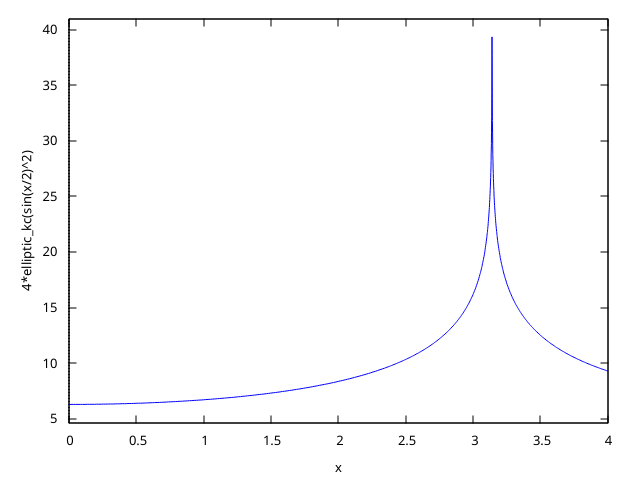
\includegraphics[scale=0.75]{images/2024-09-13-period.png}
\end{figure}


%%% Local Variables:
%%% mode: latex
%%% TeX-master: "journal"
%%% End:
